\section{Auswertung}

\section{Auswahl der NV-Zentren}
Im Versuch wurden zweimal ein NV-Zentrum und anschlie\ss end die hellste Lichtquelle analysiert.
Die Abbildungen \vref{fig:NV} und \vref{fig:hell} zeigen, wie die Messpunkte in der Probe ausgew"ahlt wurden.
\begin{figure}[htbp]
    \begin{subfigure}[t][][b]{0.43\textwidth}
        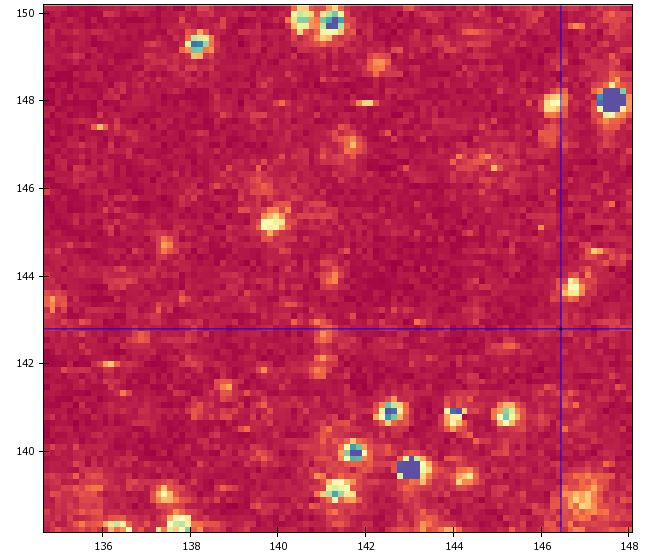
\includegraphics[width=1\textwidth]{messung_1.JPG}
        \subcaption{Messung: NV-Zentrum 1}
        \label{fig:NV:1}
    \end{subfigure}
    \begin{subfigure}[t][][b]{0.42\textwidth}
        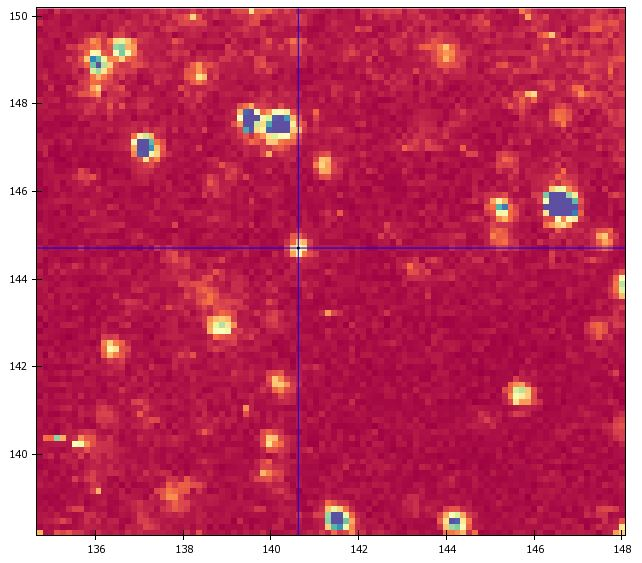
\includegraphics[width=1\textwidth]{messung_2.JPG}
        \subcaption{Messung: NV-Zentrum 2}
        \label{fig:NV:2}
    \end{subfigure}
    \hfill
    \begin{subfigure}[t][][b]{0.1\textwidth}
        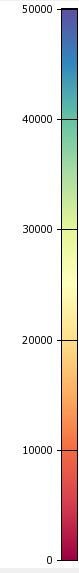
\includegraphics[height=3.6\textwidth]{skala_1_2.JPG}
    \end{subfigure}
    \caption{
        Die Abbildung verdeutlicht, wie die NV-Zentren f"ur die Messung ausgew"ahlt wurden.
        Die Graphiken zeigen dabei die Intensit"atsverteilung der Lichtemission in der Probe.
        Einzelne NV-Zentren sind diejenigen Punkte, die von den anderen separiert sind, keine zu hohe Intensit"at haben und im Zoom etwa kreisf"ormig erscheinen.
        Das blaue Fadenkreuz zeigt jeweils an, welches Zentrum f"ur die beiden Messungen ausgew"ahlt wurde.
        Die Messungen werden NV-Zentrum 1 und NV-Zentrum 2 genannt.
        Bei NV-Zentrum 1 liegt das Fadenkreuz nicht mehr ganz auf dem Punkt (rechts "uber dem Fadenkreuz).
        Dies liegt daran, dass das Bild erst am Ende der Messung aufgenommen wurde.
        Die Intensit"atsverteilung zeigt dabei die Situation zu Beginn und das Fadenkreuz die Position des NV-Zentrums nach etwa zwei Stunden.
        Es ist um einiges gewandert.
        \\
        Zur Skala: Die Angaben an den Bildern sind in \si{\nano\metre} und die Intensit"atsskala ist in \si{counts\per\second} gegeben.
        }
    \label{fig:NV}
\end{figure}
\begin{figure}[htbp]
        \begin{subfigure}[t][][b]{0.43\textwidth}
            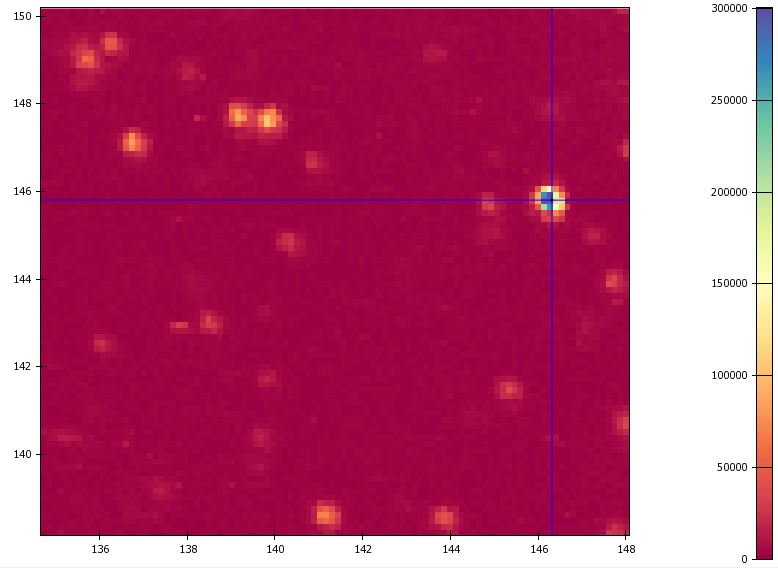
\includegraphics[width=1\textwidth]{messung_3.JPG}
        \end{subfigure}
        \hfill
        \begin{minipage}[t][][b]{0.5\textwidth}
            \caption{
                Messung: Hellster Punkt
                \\
                Zus"atzlich zu den NV-Zentren wurde noch eine weitere Lichtquelle untersucht.
                die nebenstehende Abbildung zeigt, wie der hellste verf"ugbare Punkt als Quelle ausgew"ahlt wird.
                \\
                Zur Skala: Die Angaben an den Bildern sind in \si{\nano\metre} und die Intensit"atsskala ist in \si{counts\per\second} gegeben.
                }
            \label{fig:hell}
        \end{minipage}
\end{figure}

\subsection{Berechnung der Korrelationsfunktion}
\begin{table}[htbp]
    \caption{
        Die Tabelle zeigt die Z"ahlraten $N_1$ und $N_2$ der Detektoren die zu einem Zeitpunkt w"ahrend der Messung aufgenommen wurden.
        Ihr Verh"altnis $f=N_2/N_1$ wird direkt daraus berechnet.
        Wie unschwer zu erkennen ist, arbeitet Detektor 2 effizienter als Detektor 1.
        }
    \label{tab:counts}
    \begin{tabular}{l|*2S[table-format=6]S[table-format=1.2]}
        Versuch
            &{$N_1$ [\si{counts\per\second}]}
            &{$N_2$ [\si{counts\per\second}]}
            &{$f=N_2/N_1$}\\\hline
        NV-Zentrum 1
            &11000
            &20000
            &1.82\\
        NV-Zentrum 2
            &12000
            &21000
            &1.75\\
        Hellster Punkt
            &120000
            &200000
            &1.67
    \end{tabular}
\end{table}
Im Versuch wird ein Histogramm aufgenommen, welches die H"aufigkeit z"ahlt, mit der zwischen dem Klick an Detektor 1 und dem an  Detektor 2 die Zeit $\tau$ vergeht.
Diese Verteilung wird im folgenden $c(\tau)$ genannt.
Zus"atzlich werden die Z"ahlraten $N_1$ und $N_2$ der Detektoren 1 und 2 aufgenommen.
Die aufgenommenen Z"ahlraten sind in Tabelle \vref{tab:counts} eingetragen.
Es zeigt sich, dass diese im Versuch stark variieren; beim ersten Durchgang schwankte $N_2$ zwischen \SI{10000}{} und \SI{30000}{}.
Diese Schwankung ist darauf zur"uckzuf"uhren, dass die NV-Zentren in der Probe wandern und sich so aus dem Fokus bewegen.
Dieser wird zwar alle 3 Minuten neu justiert, aber der Intensit"atsverlust ist dennoch bedeutend.
Um diese Schwankung auszugleichen, wird das Verh"altnis $f=N_2/N_1$ konstant gehalten um die Z"ahlraten anschlie\ss end so zu optimieren, dass die Korrelationsfunktion $g^{(2)}(\tau)$ f"ur gro\ss e Zeitdifferenzen $\tau$ zu $g^{(2)}(\abs{\tau}\gg \tau_\text{c})=1$ wird, wobei $\tau_\text{c}$ die Korrelationszeit ist.

